This chapter will outline how the design plans previously described have been implemented and put into play. The chapter will start with discussing how the development process has been approached, and then the system features. The chapter will conclude by describing the issues that have been raised during the process, along with how they have been resolved. A priority in this project has always been to make it as extensible and as decoupled as possible.

\section{Development Approach}
The approach to software development was dictated by the fact that the project was conducted by only one individual. As such, a lean approach was adopted, where small iterations of the project and features are incrementally implemented and integrated. 

The process has started by prototyping in order to figure out the feasibility of using certain libraries to achieve the proposed goals. Thus, the first experimental application was one that used ARKit in order to place different AR objects around Bush House in convenient location. This led to a better understanding on how ARKit will be later used and how feasible it is to implement the planned features. After this, the capabilities of Swift running on the server through the Vapor framework, and a small server that implements a REST API has been developed.

During the development process, the independence between all the parts of the system has been closely followed, along with increased re-usability and flexibility to change without affecting the whole system in any way. The order of the developed work has been decided based on the dependencies between the sub-systems and layers, considering the following points:
\begin{enumerate}
    \item Create the system where data can be stored in.
    \item Build the way that allows the system to collect data.
    \item Create the data processing units (the logic layer).
    \item Finish by integrating all the sub-systems into the front-end that is going to use the end result of the logic layer (the user application).
\end{enumerate}

Given the previous points that describe the strategy adopted, the following steps have been taken to in order to build the system. Each step describes what part has been developed, and what requirements have been satisfied.
\begin{enumerate}
    \item Create the database schema for the database objects along with their respective classes (BAPI1, BAPI2).
    \item Make the database objects accessible through a REST API. The resources necessary for the applications to retrieve data have also been developed here (BAPI3, BAPI4).
    \item Build a scanner and parser on the Raspberry Pi and an autonomous script that will run the scanning process every 2 seconds (RPS1, RPS2, RPS3).
    \item Create a Scanner Switch on a server that will notify the Raspberry Pi when the data is needed (WSS1, WSS2).
    \item Build UIViewController to view available floors that are available to measure from the Admin Application.
    \item Build UIViewController on the Admin Application that will manage adding and deleting rooms from the database (AM1, AM4).
    \item Build a UIViewController on the Admin Application to view the floor plan corresponding to the selected room. Event handlers for tapping on the screen have been created here too. This will start the scanning process by turning the Raspberry Pi on, creating a Location entity associated to a room, and then the data that has been scanned from the Wi-Fi networks around will be assigned to that Location (AM3).
    \item Create the event handler for the Admin Application to connect two Location entities. The link between them will make navigation possible. This concludes data collecting, which gives way to develop the positioning algorithm (AM3).
    \item Implement the path finding algorithm by using Dijkstra's algorithm, and the positioning algorithm (BS1, BS2).
    \item Create the UIViewController on the User Application that shows the user's location in the correct floor and room (UM1)
    \item Create  UIViewController that shows all available rooms to select as destinations, along with a way to search for them (UM2, UM3).
    \item Show the path calculated from the server on the User Application, with its respective distance and estimated time arrival (UM4, UM5).
    \item Create the button to switch to the AR mode; this will show an arrow when the user is currently navigating to a destination (UM6).
    \item Implement the parser to get timetables from King's College London Timetable service (ARDP1).
    \item Implement the parser to get the number of computers in computer labs from PC-Free@King's (ARDP2).
    \item Build the UIViewController on the User Application that will allow the user to see augmented reality objects of timetables of the rooms around (UM7).
    \item Build the UIViewController on the User Application to show the number of unused computers of the rooms around, if available (UM8).
\end{enumerate}

\section{System Functionalities}

This section will describe how each part of the system has been implemented and developed. It will start by outlining the lowest layer, the Data Management Layer, and it will conclude with the upper most layer, the User Interface Layer. The core functions for each layer will be portrayed in detail, along with pieces of code where needed.

\subsection{Data Management Layer}
\subsubsection{Database}
Initially, the database has been implemented by using SQLite3, but because of deployment issues on Heroku, it has been changed to PostgreSQL. The first models to be created in the database have been Room and Location. After the design phase, the following models have been created:

\noindent
\textbf{Room: }This is the entity which lays at the base of all the other models. It follows the model outlined in the Design chapter 4, section \ref{sec:data-storage-objects}.
\begin{lstlisting}
roomName: String, floorNumber: Int, id: Identifier
\end{lstlisting}

\noindent
\textbf{Location: }This entity belongs to a Room and describes a single location in a room. It has 2 sets of coordinates, because a Location is based into 2 coordinates system: 2D (on the floor plan), and geographic (latitude and longitude). The 2D coordinates is used in order to place a Location object on the mobile phone's screen, and the geographical ones are used for navigation purposes. Between a Room and a Location there is a one-to-many relationship (a Room has many Locations), and a Location must belong to a Room.
\begin{lstlisting}
x: Double, y: Double, standardWidth: Double, standardHeight: Double,
latitude: Double, longitude: Double,
roomID: Int,
id: Identifier
\end{lstlisting}

\noindent
\textbf{Measurement: }This entity contains only the signal strength part of a network scan. The initial implementation included the access point from where the signal was collected, but in order to avoid duplication, the two entities have been separated through a one-to-many relationship from Access Point to Measurement. Finally, a Location is connected to Measurements through a one-to-many relationship.
\begin{lstlisting}
signalStrength: Int, accessPointID: Int, locationID: Int
\end{lstlisting}

\noindent
\textbf{Wi-Fi Access Point: }This entity describes the Wi-Fi Access Point from where the Measurements have come from.
\begin{lstlisting}
name: String, macAddress: String
\end{lstlisting}

\subsubsection{REST API}
The REST API has been implemented using Vapor which relies on Swift. HTTP requests have been handled using the HTTP module under Vapor. JSON encoding and decoding have been made using the JSON module under Vapor, as well. The resources and endpoints used to access the database for CRUD operations have been implemented by following the points described in the Design section.

\subsection{Logic Layer}
\subsubsection{Positioning \& Path Finding System}

This system has been implemented using Vapor and by using Swift. The system relies on just two classes – a PositionCalculator and a NavigationEngine, which will be described into detail in the following sections. In order to access the functionalities of these classes, several endpoints have been developed.

\subsubsection*{PositionCalculator.swift}
This class is responsible for calculating the user's current position, based on a set of Measurements received in a JSON format. The class is a singleton and inherits from NSObject, which is the class that has base functionalities in Swift.
Calculating the position starts by sending a JSON array which has network names, MAC addresses and signal strengths from the scanned networks. The JSON data is included in a  POST HTTP request made to "/calculatePosition", from the Java application that runs on the Raspberry Pi. A sample scan result in JSON format is: 
\begin{lstlisting}
[
    {"macAddress":"00:62:EC:FD:EC:50","signalStrength":-62,"name":"eduroam"},
    {"macAddress":"00:62:EC:FD:ED:72","signalStrength":-59,"name":"The Cloud"},
    {"macAddress":"00:62:EC:FD:EC:C2","signalStrength":-64,"name":"KINGSWAP"},
    {"macAddress":"00:62:EC:FD:EB:14","signalStrength":-63,"name":"SLaMFT"}
]
\end{lstlisting}

The following step is to parse the data received, and to call the determinePosition(for measurementsCollection) in the calculator, which returns a Location object. 
\begin{lstlisting}
func determinePosition(for measurementsCollection: MeasurementsJSONCollection) -> Location?
\end{lstlisting}

The method follows the methodology outlined in Section 4.1.3.1. It starts by initialising a dictionary object, "locationMarks", which will store the number of matches a locationID has. In other words, the keys will be location ids that have resulted in calculation, and for any location id, the result retrieved will be the number of matches. Next, a loop will iterate through the measurementsCollection, and for each measurement, the MAC address and the network's name will be extracted and used to query for old measurements from the database. The following code is the implementation of this:
\begin{lstlisting}
var locationsMarks = [Int: Int]()

    for currentScanMeasurement in measurementsCollection.measurements {
        let currentScanMacAddress = currentScanMeasurement.macAddress
        let currentScanSignalStrength = currentScanMeasurement.signalStrength

        guard let searchResults = searchForOldMeasurements(for: currentScanMacAddress)?.results else { print("Not found!"); continue }
\end{lstlisting}

Following this, another loop iterates through the searchResults, and for each result, calculates the following difference:
\begin{align}
    difference = |(currentScanSignalStrength * -1) - (result.signalStrength * -1)|
\end{align}

Because the signal strengths are received in negative values, in order to get the correct difference between them, they are multiplied by -1 to get their positive value and then the end result is taken in its absolute value. The following step is to find if this difference is smaller than the ones recorded before the current step for this search result, and if it is, store its locationID.

\begin{lstlisting}
for result in searchResults {
    let diff = abs((currentScanSignalStrength * -1) - (result.signalStrength * -1))
    if diff < minDiff {
        minDiff = diff
        minLocationID = result.locationID
    }
}
\end{lstlisting}

At the end of the for-loop that iterates through the searchResult, for the locationID that had the smallest difference between its measurements and the scanned measurements, its matches value is increased in the dictionary.

\begin{lstlisting}
if locationsMarks[minLocationID] != nil {
    locationsMarks[minLocationID] = locationsMarks[minLocationID]! + 1
} else {
    locationsMarks[minLocationID] = 1
}
\end{lstlisting}

The last step is to find which locationID has the most matches, and return the corresponding Location object for that locationID.

\begin{lstlisting}
for (key, value) in locationsMarks {
    if value > maxMatches {
        maxMatches = value
        locationID = key
    }
}

guard let location = getLocationDetails(for: locationID) else { return nil }
return location 
\end{lstlisting}

The result is then encoded into a JSON format of the Location object. Additional fields have been added in order to have additional information in the user application, such as:
\begin{itemize}
    \item A "success" field which is true if the calculation was successful, or false if it failed.
    \item "floorNumber" which will help the user application show the correct floor plan.
\end{itemize}

A sample result of a positioning calculation will look like this:
\begin{lstlisting}
{   
    "roomID": 2, 
    "latitude": 51.5124257954173, 
    "standardHeight": 1024, 
    "id": 3, 
    "floorNumber": 7, 
    "x": 348.5, 
    "longitude": -0.117183612390869, 
    "y": 862.5, 
    "standardWidth": 768, 
    "success": 1
}
\end{lstlisting}

\subsubsection*{NavigationEngine.swift}
This class is responsible for calculating routes between any two given Locations. Same as before, the class inherits from NSObject and is a singleton. Calculating a route starts by a POST HTTP request to "/calculateRoute". The input received is a JSON object that has only two values: the location ID of the starting point and the location ID of the finishing point. This JSON object is parsed by a HTTP requests handler class in the application, data is fetched from the database to receive more information about the two locations, and then the process starts. The below input is a sample input received by the server:

\begin{lstlisting}
{
    "startLocationID": 1,
    "finishLocationID": 24
}
\end{lstlisting}

After the input has been parsed, the process will create the graph which Dijkstra's algorithm will use. The first step towards creating the graph was to create the data structures that will act as nodes as edges. The data structure for nodes has already been created, which is the Location entity, but for edges, the following data structure has been built:

\begin{lstlisting}
struct Edge: Decodable {
    let rootLocationID: Int
    let childLocationID: Int
}
\end{lstlisting}

The structure inherits from "Decodable" which is an interface that allows a JSON format to be transformed into an instance of the structure. Taking this into account, the next step is to get the connections between all the Locations; in other words, the edges between them. The edges are stored into a dictionary $edges$, where $edges[locationID]$ is an array of locationIDs that belong to Locations connected. The code below depicts what has been said: first, all the Locations are fetched, and for each Location, the connections are fetched and the graph is assembled.

\begin{lstlisting}
func createGraph() {
    guard let locations = NetworkingHelper.shared.fetchAllLocations() else { return }
    self.locations = locations // the result is saved into a global variable
    
    for location in locations {
        let id = location.id
        distance[id] = INF // For each locationID, the array of distances which will be later used is initialised; in other words, the distance is infinite => it's unreachable
        prev[id] = 0 // Same for the array of parents; the initial value is set to 0, in other words, the location does not have a parent for now

        guard let currentEdges = NetworkingHelper.shared.getEdges(for: location.id) else { continue }

        for edge in currentEdges {
            // If the array of ids has not been initialised, the initialisation happens here
            if edges[edge.rootLocationID] == nil {
                edges[edge.rootLocationID] = [Int]()
            }

            // The child's locationID is appended here to the array of connections in the dictionary
            edges[edge.rootLocationID]!.append(edge.childLocationID)
        }
    }
}
\end{lstlisting}

Next, after the graph has been created, the value in the $distance$ corresponding to the starting point is updated to 0, the node is set as visited, and the priority queue is initialised. Before the algorithm starts, the starting node is added into the priority queue. The following code describes the main process of the function:

\begin{lstlisting}
while(!queue.isEmpty) {
    guard let node = queue.remove() else { break } // Removes the first node in the queue; to avoid force unwrapping the value which causes a crash, a guard-let structure is used
    visited[node] = false // First set its value as not visited
    if let edges = edges[node] { // Again, avoid force unwrapping
        for neighbour in edges { // Iterate through all the node's neighbours
            if let dist = distance[node] { // Unwrapping it's distance
                let alt = dist + getDistance(from: node, to: neighbour) // Compute the alternative distance
                if let neighbourDistance = distance[neighbour] { // Unwrapping the neighbour's current distance
                    if alt < neighbourDistance { // Checking if the previously calculated distance is better, and if it is, replace it and add the node in the queue
                        distance[neighbour] = alt
                        prev[neighbour] = node // Add the node as the neighbour's parent
                        queue.insert(neighbour)
                    }
                } else {
                    distance[neighbour] = INF // If it's value is null, initialise to INF.
                }
            } else {
                distance[node] = 0 // Set it to 0 if it's null.
            }
        }
    }
}
\end{lstlisting}

An important point to discuss here is how distance is calculated. Because the Location object already stores the latitude and longitude values, it is therefore easy to calculate the real life distance between them. This uses the haversine formula previously described in section \ref{sec:haversine}. This function is already implemented in the Foundation framework which Swift uses. The Foundation framework provides access to essential data types, collections and others, that define the base layer of any Swift based application. 

The last step of the algorithm is to create the path by backtracking it, using the $prev$ array. As stated in the Background section, this array stores an element's parent; in other words, for $prev[v] = p$, where $p$ is the parent of $v$. The path will be backtracked from the destination to its start.

\begin{lstlisting}
func createPath(parentsList: [Int: Int], distances: [Int: Double], start: Int, finish: Int) -> [String: Any]? {
    if distances[finish] == INF { // If the distance for the destination is infinite, that means it has never been reached.
        return [
            "sucess": false
        ]
    }
    
    var path = [Int]()
    var currentNode = finish
    path.append(currentNode)
    while (currentNode != start) {
        if parentsList[currentNode] != nil {
            path.append(parentsList[currentNode]!)
            currentNode = parentsList[currentNode]!
        }
    }
        
    return [
        "success": true,
        "distance": distances[finish]!,
        "path": path.reversed() as [Int] // This array has all the locationIDs to follow.
    ] as [String: Any]
}
\end{lstlisting}

The end result after creating the path is then encoded into JSON format and returned to the mobile phone. The JSON object will have the distance of the path, the array of locationIDs and a success field which role is to inform the client if the calculation has been successful or not.

\begin{lstlisting}
{
    "success": true,
    "path": [
        1,
        3,
        13,
        15,
        16,
        18,
        20,
        21,
        24
    ],
    "distance": 78.4722368482206
}
\end{lstlisting}

\subsubsection{AR Data Provider}

The initial design of this system was to be included in the one system, together with the Positioning \& Path Finding system. However, due to the lack of a web automation library that in combination with a parser will retrieve data, these two systems have been separated instead.

Instead of Vapor and Swift, this system has been written in Python, using Selenium, an automation tool for browsers. Next, the software has been deployed to work through a server with a lightweight API to access data. The framework used for deploying it and API management is Flask, which allows to do web development using Python.

\subsubsection*{Timetable information}
Getting timetable information for a specific room starts with a GET HTTP request to "/timetable/:room", where ":room" is the room code (e.g. 6.01 is computer lab 1 on the sixth floor in Bush House). 

The way the provider works is fairly simple. Using Selenium, Chrome is launched on the server, then the web browser navigates to "http://timetables.kcl.ac.uk". From here, the Locations module of the timetable website is accessed. This shows a form that is going to be filled in automatically with the required data in order to obtain the desired timetable.

\begin{figure}[H]
    \centering
    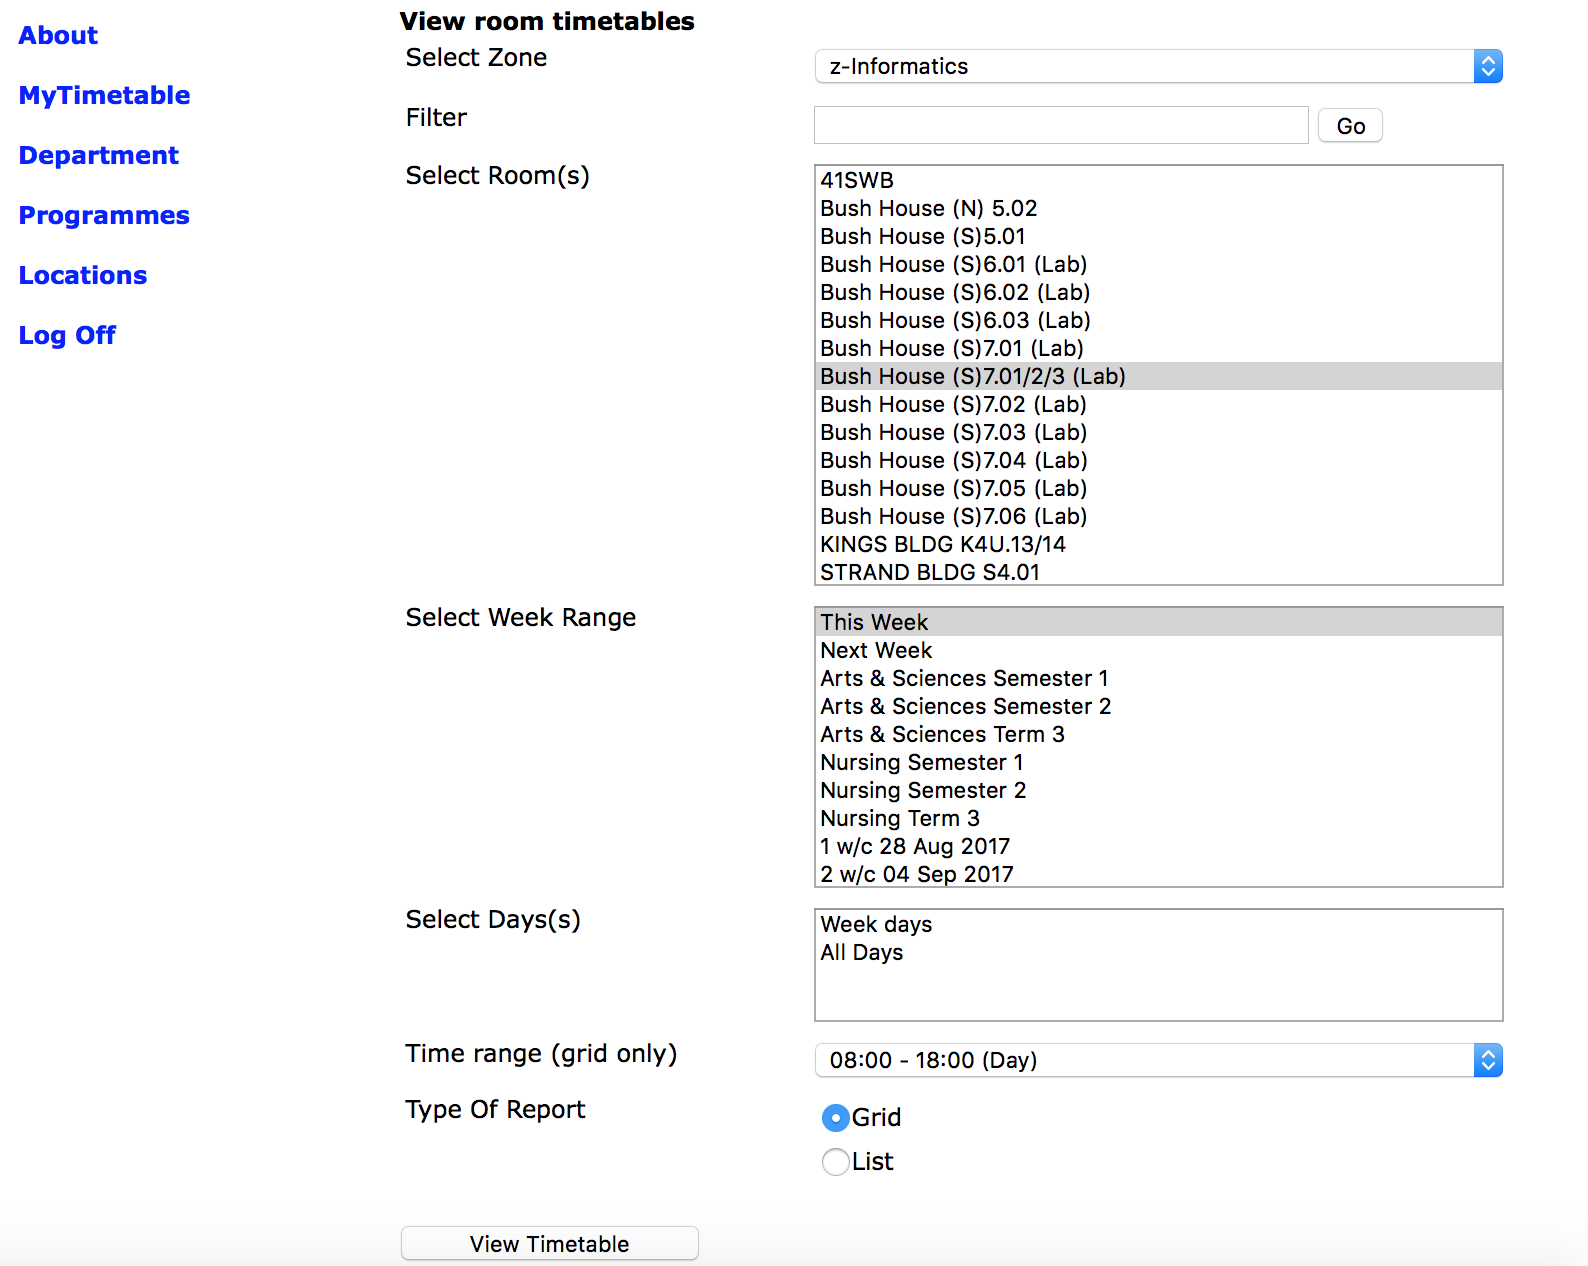
\includegraphics[width=420px, height=335px]{Implementation&Testing/timetable.png}
    \centering
    \caption{KCL timetable with form to choose rooms. This is the standard form where students can put information to see the timetables. This will be filled in automatically by the Python script with the necessary information, and the "View Timetable" button will be pressed at the end.}
\end{figure}

The end result will be a screen-shot with the timetable for the requested room. The image will be set as background for an augmented reality object in the user application. Next, it will be placed in the closest Location that belongs to the requested room, from the user's current position. This process will be further detailed in the section for the user application.

\begin{figure}[H]
    \centering
    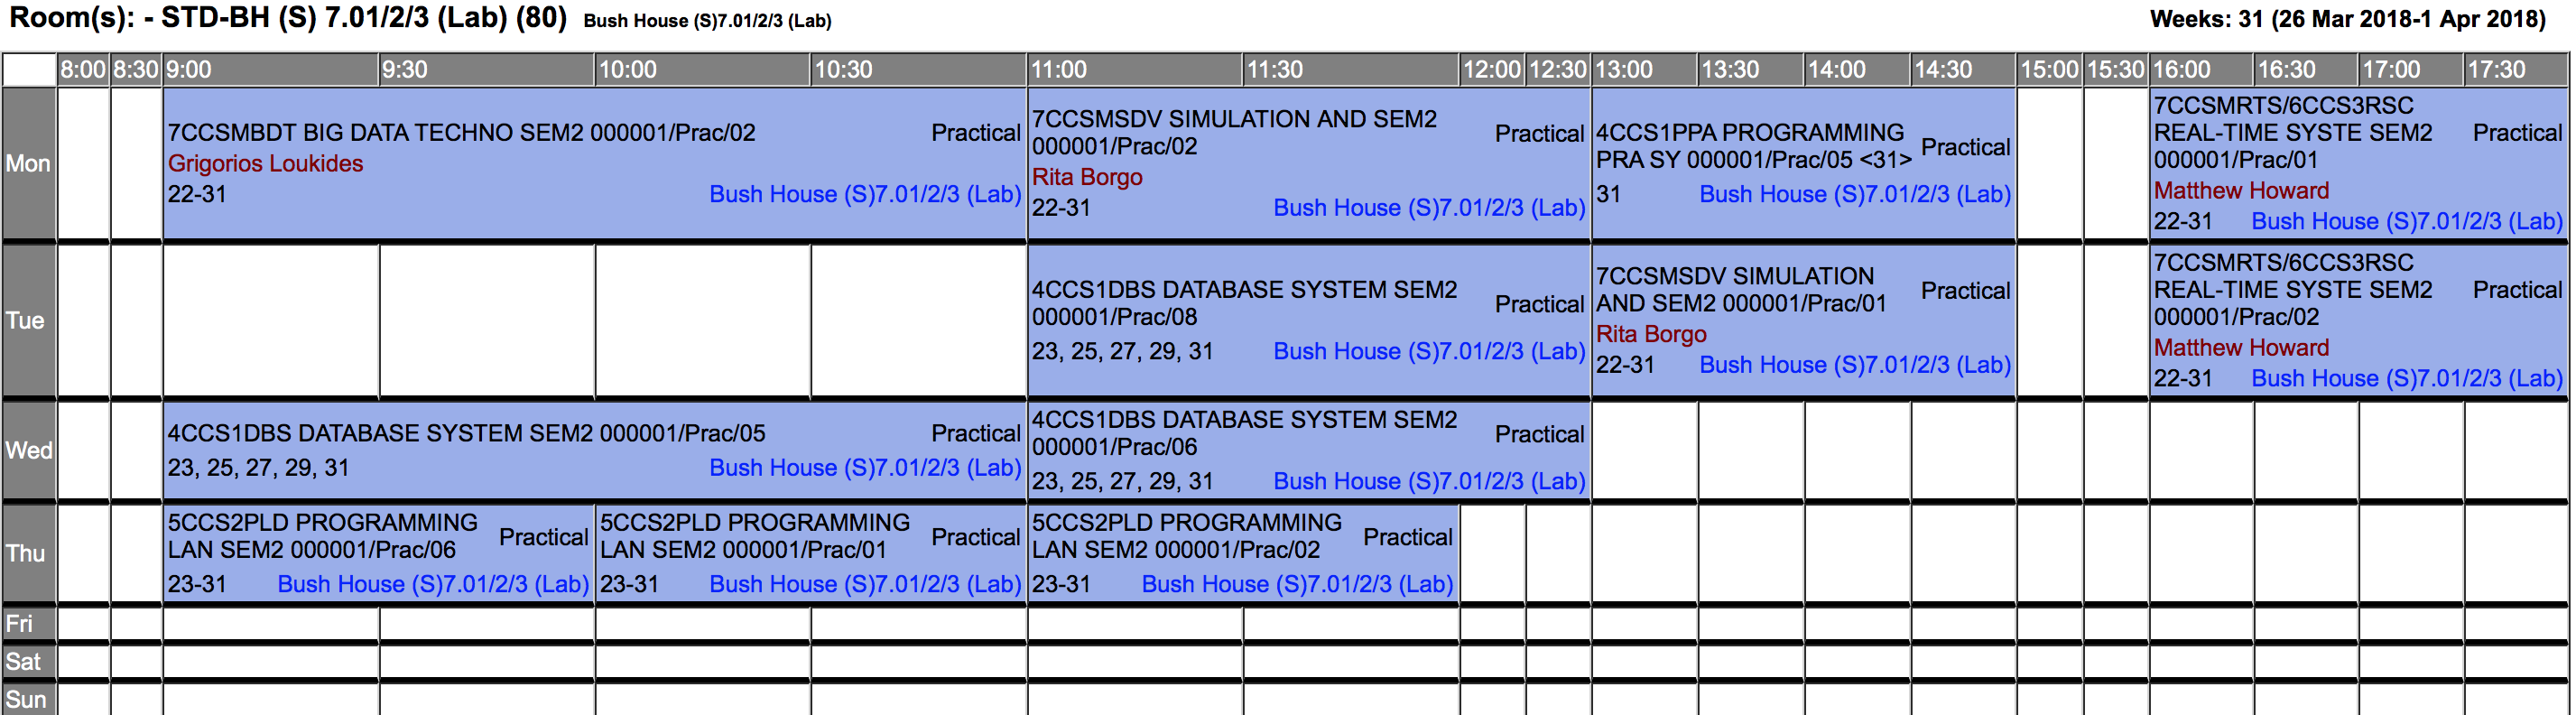
\includegraphics[width=420px, height=117px]{Implementation&Testing/timetable-701.png}
    \centering
    \caption{Sample timetable for room 7.01/2/3. This is the result of the form shown in figure 5.1.}
\end{figure}

\subsubsection*{PC-Free information}
The PC-Free provider works in a similar way as the timetable one. To access data for a room, a GET HTTP request is made to "/pcfree/:room", where as before, ":room" is the code of the room. The web driver then navigates to "http://pcfree.kcl.ac.uk", and searches for the element that matches the room for which the data was requested. Once found, a screen shot is taken from the whole screen, and then cropped around the area of interest.

\begin{lstlisting}
def get_available_computers(room):
    for element in driver.find_elements_by_class_name('campus_info'):
        square = element.get_attribute('innerHTML')
        bs = BeautifulSoup(square, "html.parser")
        full_room_name = bs.find('h2').text
        if "BH(S)" in full_room_name:
            if room in full_room_name:
                location = element.location
                size = element.size
                img = driver.get_screenshot_as_png()
                img = Image.open(BytesIO(img))
                left = location['x']
                top = location['y']
                right = location['x'] + size['width']
                bottom = location['y'] + size['height']
                img = img.crop((int(left), int(top), int(right), int(bottom)))
                img.save('pcfree.png')
                return
    return None
\end{lstlisting}

The result is encoded into JSON format, and then sent to the requesting entity.

\subsection{Scanning Layer}
\subsubsection{Raspberry Pi Scanner}
The scanner on the Raspberry Pi is composed of a bash script that scans continuously for Wi-Fi networks, and then runs a Java application that parses the results and uploads them if needed. In order to perform a scan, the system uses a Linux package, iwlist, and then the results are manipulated by grep, that matches them to a regular expression.
\begin{lstlisting}
sudo iwlist wlan0 scan | egrep "Cell|ESSID|Signal" >> output.txt
\end{lstlisting}

\noindent
Next, the Java application is started using Maven. The application will first check from the Scanner Switch if data is needed. If it is, it will parse the output file, and upload them either to the database, if data is needed for measuring, or temporarily uploads them on the Switch server, if data is used for navigation. The process ends by deleting the output file in order to make room for the next scan.

It is important to mention that the scanning process starts at boot time. After the Raspberry Pi boots, the script described earlier runs every two seconds, until the shut-down of the device.

\subsubsection{Scanner Switch Web Application}
This web application is positioned between the mobile applications and the Raspberry Pi scanner. This connection was initially planned to happen directly between the mobile devices and the Raspberry Pi via Bluetooth, but due to the difficulties encountered and the time constraints, this new design has been adopted. It is important to say however, that given the architectural design which is very loosely coupled, this connection type can be changed at any time. The web application is implemented using Vapor and Swift. It contains only two classes, which are ScanSwitch and Measurement. 

\subsubsection*{ScanSwitch.swift}

The Scan Switch class acts as a physical switch that stores boolean flags that need to be checked by the Raspberry Pi in order to trigger a scan. 

\begin{lstlisting}
shouldScan: Bool
roomID: Int
locationID: Int
storeData: Bool
\end{lstlisting}

\noindent
Other than the shouldScan flag, ids for rooms and locations are temporarily stored too. These are used to make the connection between the measurements collected by the scanner with first the Location and then the Room. Lastly, the storeData flag is used by the Java application that decides where to upload the data: the measurements database, or temporarily on the scanner web application.

\subsubsection*{Measurement.swift}
This class is identical to the one described for the server that manages the database. In order to avoid repetition, its fields and properties will not be included. As previously mentioned, this class is used to temporarily store data that is used for positioning. After the positioning process ends, the data is discarded.

\subsection{User Interface Layer}
The User Interface Layer is an important component, because it acts as the primary way for the user to interact with the system. The graphical user interface provides a clear and simple way to measure floor plans, see recorded locations, manage rooms or navigate through the building. The implementation choices and features for each mobile application will be described in the following sections.

\subsubsection{Admin Application}
The Admin Application is implemented as an iOS application, written in Swift. It follows an Model-View-Controller pattern design, which is standard on iOS. The classes included in the mobile application are mainly used to make HTTP requests to ask for data, and then the View Controllers handle showing data onto the screen. Some simple calculations are being made in order to calculate the latitude and longitude coordinates, given the floor plan coordinate values.

\subsubsection{Model classes}
The model for this application is composed of a Location class, which is identical to the class in the server that manages the database, and is used in order to download or upload user locations. In order to avoid repetition, it will not be detailed further. The rest of the model classes are HTTPClient and Utils.

\subsubsection*{HTTPClient.swift}
This class manages all HTTP requests that are being made in the app. Its design is very simple, it is based on a singleton design pattern, and contains only one method which is able to make any type of HTTP requests. The method uses URLConnection, which runs asynchronously on a background thread in order to not block the user interface thread. The method can submit a JSON object in the HTTP request if needed, and if there is a JSON object as a response, it will return it.

\subsubsection*{Utils.swift}
This class contains utility functions which are used along the app in order to do small calculations. All of the calculations are geometry based, such as the haversine distance, the Manhattan distance, a circle intersection, and point coordinates interpolation. The following paragraphs will highlight how these functions are performed.

\subsubsection*{Haversine Distance}
The Haversine has been mathematically detailed in the Background chapter. The code implements the aforementioned equations, and it is taken from the Swift Algorithm Club. The credit for this code has clearly stated in the class file.

\begin{lstlisting}
let haversin = { (angle: Double) -> Double in
	return (1 - cos(angle))/2
}
		
let ahaversin = { (angle: Double) -> Double in
    return 2*asin(sqrt(angle))
}
		
// Converts from degrees to radians
let dToR = { (angle: Double) -> Double in
    return (angle / 360) * 2 * Double.pi
}
		
let lat1 = dToR(la1)
let lon1 = dToR(lo1)
let lat2 = dToR(la2)
let lon2 = dToR(lo2)
		
return radius * ahaversin(haversin(lat2 - lat1) + cos(lat1) * cos(lat2) * haversin(lon2 - lon1))
\end{lstlisting}

\subsubsection*{Circle Intersection}
Circle intersection is being made between the corners of the building and the desired location that the admin wants to register. The values of latitude and longitude for all four corners of the building (top right/left, bottom right/left) are being loaded into the app, and then at launch, the user is put to register the locations of these corners in the 2D plan, by tapping on the screen. Based on this association of values, the distances are then calculated in the following way:
\begin{enumerate}
    \item Two corners are chosen, and the distance between the desired location and each of those two corners is calculated using the Manhattan distance.
    \item The hypotenuse of the triangle formed between these three locations is calculated.
    \item The set of equations is therefore solved and the possible two intersections are returned.
\end{enumerate}

It is important to mention that the solution is based on an external source which has been adapted to the current needs of the application. The source of the algorithm has been clearly specified in the source code. Please refer to the Appendix for more details.

After the intersection is performed, the Location object can then be uploaded into the database, with its 2D location and its latitude and longitude. The latitude and longitude positions are used for navigation, in order to find the distance, and to place augmented reality objects.

\subsubsection*{Interpolating 2D Coordinates}
Location objects are being registered on different screen sizes. For example, the iPad is used for measuring, because the larger screen makes it more accurate when tapping on the floor plan image. Because of this, the coordinate set changes for each device the application runs on. In order to show the same position on the screen no matter what the size of the screen is, the 2D coordinates have to be adapted, based on the device they have been registered on. Therefore, the points are interpolated based on the standard size (the source) and the current size of the screen. The code below illustrates this better.

\begin{lstlisting}
static func interpolatePointToCurrentSize(point: CGPoint, from standardSize: CGSize, in view: UIView) -> CGPoint? {
	let currentSize = view.bounds.size // Getting the current size
	return CGPoint(
		x: point.x * currentSize.width / standardSize.width,
		y: point.y * currentSize.height / standardSize.height
	) // Calculate it based on the registered size and the current one and return the corresponding CGPoint.
}
\end{lstlisting}

\subsubsection{View Controller classes}
This is the iOS application which will be used by administrators to manage rooms. The calibration process is achieved by asking the user to tap on the image on the top left \& right and bottom left \& right corners of the floor plan's image. This calibration is done in the CornerViewController class, and the values are saved in the UserDefaults persistent storage. 

After calibration is done, view controllers that are handling rooms managing and location managing are being launched. These will be further illustrated below.

\subsubsection*{InitialViewController}
This is the entry view controller of the app. It was built in order to decide whether the app needs calibration (in other words it is the very first launch), or not. From here, the CornerListViewController or the FloorListViewController are launched.

\subsubsection*{CornerListViewController}
This class implements a UITableView for the user to choose what corner they wish to register. From here, tapping on one of the options will launch another ViewController, with an image of the floor plan. Tapping on the required corner will save the data locally, as previously mentioned.

\subsubsection*{FloorListViewController}
Similarly to the CornerListViewController class, this class implements a UITableView as well. The list contains the floor that are in the Informatics deparment in Bush House, which are level 5, 6 and 7. Tapping on one of them will launch another view controller of the list of rooms registered on that floor.

\subsubsection*{RoomListViewController}
This class implements a UITableView which is filled in with the rooms on the selected floor. From here, the user can add a room by pressing a "+" button and filling in the data, delete a room or clear the data from it. By pressing on a room, this will launch an image of the floor plan, from where the user can record locations. The methods available in this class use the HTTPClient class to make HTTP requests to the database, in order to perform CRUD operations.

\subsubsection*{FloorPlanViewController}
This is the last and most important view controller in the app. It implements an UIImageView which shows the floor plan for the selected floor. Upon loading, the already registered locations are placed on the floor plan by fetching them from the database. User can tap on the image on the locations where they need to register a location. Next, a request is made to the Scanner Switch to scan data with the roomID and locationID of the Location just created, and the measurements will be uploaded from the Raspberry Pi to the database. 

Additionally, this view controller allows admins to connect to Locations, which helps in the  navigation process. This is done by tapping on one Location square from the screen, which is set as the root location. The next step is to tap the location to connect the current one to, which is set as the child. After both have been selected, a HTTP request is made to the database through the REST API, and a LocationConnection entity is created.

\subsubsection{User Application}
This is the iOS application which will help users to find where they are in the building, how to get to certain other rooms and to find information about the rooms around them, such as timetables. In the implementation of this application, some model classes have been reused from the admin application or the database, such as Room or Location, or the HTTPClient.

The implementation of the application of the application consists of a model which mainly consists of helper classes that make HTTP requests to different APIs. To get the full implementation of them, please refer to the Appendix. In the following paragraphs, the most important parts of the application implementation will be highlighted.

\subsubsection{Model classes}
\subsubsection*{IndoorLocationManager.swift}
As previously mentioned in the Design chapter, the application uses an external library (ARKit + CoreLocation) to place augmented reality objects in certain locations, given their latitude and longitude. By default, this library uses CoreLocation, which is a library part of iOS which manages locations. Because this library uses the mobile phone's GPS or GLONASS chips to determine the location. However, this defeats the purpose of an IPS, so a new location manager has been developed, that uses the system built to navigate indoors. 

The location manager is composed of an interface that lets classes subscribe to location changes, and a few methods to start or stop updating the location, and a private method to determine the current position. Determining the position is being made by making HTTP requests first to the Scanner Switch to turn it on and to get the measurements recorded, and then to the Navigation System in order to determine the current position. Please refer to the Appendix to get the full implementation of this class.

\subsubsection*{Utils.swift}
This class is similar to the one from the admin application. The methods defined here are for mathematical calculations, such as interpolating two coordinates set, which we have seen in the admin application, and to find the bearing between two Locations. The bearing is used for the AR part of the application, when an arrow will point to the direction that the user needs to follow in order to get to the destination. The implementation is based on a StackOverflow answer, which is stated in the source code.

\subsubsection{View Controller classes}
\subsubsection*{InitialViewController.swift}
This view controller is the main entry of the application. On loading, it calculates the user's current position using the IndoorLocationManager, and loads the corresponding floor plan, based on the user's location.

\subsubsection*{MapViewController.swift}
This view controller is composed of an UIImageView of the floor plan, where the user's location will be shown. The top part contains two UIButtons, from where the user can get to the DestinationViewController, which allows them to choose a destination, or to switch to the AR mode.

Upon selecting a destination, a path will be drawn on the screen from the user's current position, to the destination. This is performed using CoreGraphics, a framework part of iOS which aids with drawing basic elements. First, the application will iterate through all the points which are part of the path, and will draw a line between each two of them, in order. The following code illustrates the drawing function:

\begin{lstlisting}
func addLine(fromPoint start: CGPoint, toPoint end: CGPoint, in view: UIView) {
	let line = CAShapeLayer()
    let linePath = UIBezierPath()
    linePath.move(to: start)
    linePath.addLine(to: end)
    line.path = linePath.cgPath
    line.strokeColor = UIColor.red.cgColor
    line.lineWidth = 1
    line.lineJoin = kCALineJoinRound
    view.layer.addSublayer(line)
}
\end{lstlisting}

\subsubsection*{DestinationsViewController.swift}
This view controller has been implemented using a UITableView and a UISearchController. The UITableView shows all the rooms available on the current floor, which are fetched using the SearchHelper. The UISearchController is composed of a search bar which sits at the top of the table and is used to query the database for matching results, using again the SearchHelper. Selecting one room will bring the user back to the MapViewController, from where a path will be drawn on the screen, as previously described.

\subsubsection*{ARNavigationViewController.swift}
This view controller is the first one part of the AR mode, and aims to help users navigate, by showing an AR object made of an arrow, which points to the direction they need to follow. In order to know which direction the arrow needs to point to, the bearing angle between the current position and the destination position is calculated. This is done by using the latitude and longitude and values. Values from the mobile phone's compass are continuously received and used to rotate the arrow based on the user's orientation.

\subsubsection*{ARLocationInformationViewController.swift}
The second part of the AR mode is made of this view controller, which shows timetable information and the availability of computers in the computer labs that are close to the user's current position. First, the mobile app requests the closest locations in each room, based on the current position, and then it requests information for each of them. Images are returned for the timetables, and a JSON with the availability of the computers is returned from PC-Free. This is done using the AR Data Provided. Finally, the AR elements are placed using the ARKit+CoreLocation library, using the latitude and longitude values received from the back-end server.

\section{Testing}
In order to deliver quality solutions and products, the software produced needs to be thoroughly tested. The system developed is composed of a multitude of components and subsystems. Each of them need to tested individually, and then as a whole, to ensure that they run correctly.

\subsection{Unit Testing}
Unit testing is usually used to guarantee that the methods part of a component are producing the intended results. These kinds of tests are important when used to test a system in an isolated way, especially when they interact with other systems, because they can detect where the problem comes from. 

All the model classes that are part of the server that manages the database have benefited from unit testing. These tests have made sure that given an input, they create the right entity, with the right values. The same strategy has been applied to the Scan Switch server, which temporarily stores scanning data used for path finding. 

The positioning system has initially been tested manually, but to ensure that it runs correctly, unit tests have been created in order to check that the user is positioned correctly. For the path finding algorithm, the HTTP client has been replaced with a mock one, that returns manually created data. This data is composed of real world location from across the globe, with set latitude and longitude values. The connections between these locations have been also created manually, in order to test if the route between two of them is chosen correctly. In the graph created, there are multiple ways to navigate from point A to point B, all with different distances. In other words, the test had made sure that the route chosen is the one with the shortest distance.

\subsection{Integration between mobile applications and servers}
The mobile applications are very UI heavy, because the models are part of the servers. This is usually harder to test by unit testing. Therefore, testing these apps has been done manually, by making sure that the visual elements are placed in the right positions, and the data that they show is right. Moreover, to ensure the integration between the apps and the servers, which is done through the multitude of REST APIs, all the resources that can be accessed through the REST APIs have been thoroughly tested using Postman (an API development environment, which allows API testing). 
